% List of figures and tables to be used
%
% 1) Clustering as a function of different bins in redshift and stellar masses
%
% 2) Weak lensing signal measurement for each of these bins (?!)
% 3) Posterior distribution of astrophysical parameters
% 4) Posterior distribution of cosmological parameters
% 5) Posterior distribution of HOD, satellite fraction, 
%
%
%
%
%
%%%%%%%%%%%%%%%%%%%%%%%%%%%%%%%%%%%%%%%%%%%%%%%%%%%%%%%%%%%%%%%%%%%%%%%%%%
% HEADER
%%%%%%%%%%%%%%%%%%%%%%%%%%%%%%%%%%%%%%%%%%%%%%%%%%%%%%%%%%%%%%%%%%%%%%%%%%

\pdfoutput=1

\documentclass[iop, apj]{emulateapj}

\usepackage{xspace}
\usepackage{amsmath}
\usepackage{framed} 
\usepackage{txfonts}
\usepackage{epstopdf} 
\usepackage{color}
\usepackage{rotating}
\usepackage{natbib}
\usepackage{ulem}
\usepackage{xspace}
\usepackage{comment}
%\usepackage{hyperref}

\newcommand{\mt}[1]{{\textcolor{blue}{#1}}}
\newcommand{\hm}[1]{{\textcolor{red}{#1}}}
\newcommand{\sm}[1]{{\textcolor{magenta}{#1}}}
\newcommand{\rachel}[1]{{\textcolor{green}{#1}}}
\newcommand{\rfix}[1]{{\textcolor{cyan}{#1}}}
\newcommand{\jcap}{JCAP}

%\hypersetup{
%  colorlinks   = true, %Colours links instead of ugly boxes
%  urlcolor     = black, %Colour for external hyperlinks
%  linkcolor    = black, %Colour of internal links
%  citecolor   = black %Colour of citations
%}

\slugcomment{To be submitted to the Astrophysical Journal}

\special{papersize=8.5in,11in}
\setlength{\pdfpageheight}{\paperheight}
\setlength{\pdfpagewidth}{\paperwidth}
\newdimen\hssize
\hssize=8.4truecm

%%%%%%%%%%%%%%%%%%%%%%%%%%%%%%%%%%%%%%%%%%%%%%%%%%%%%%%%%%%%%%%%
% Text markup
%%%%%%%%%%%%%%%%%%%%%%%%%%%%%%%%%%%%%%%%%%%%%%%%%%%%%%%%%%%%%%%%

\def\red{\color{red}}
\def\blue{\color{blue}}

%%%%%%%%%%%%%%%%%%%%%%%%%%%%%%%%%%%%%%%%%%%%%%%%%%%%%%%%%%%%%%%%
% Physical units
%%%%%%%%%%%%%%%%%%%%%%%%%%%%%%%%%%%%%%%%%%%%%%%%%%%%%%%%%%%%%%%%

\newcommand{\pc}{\>{\rm pc}}
\newcommand{\kpc}{\>{\rm kpc}}
\newcommand{\mpc}{\>{\rm Mpc}}
\newcommand{\gpc}{\>{\rm Gpc}}
\newcommand{\kpch}{\>{h^{-1}{\rm kpc}}}
\newcommand{\mpch}{\>h^{-1}{\rm {Mpc}}}
\newcommand{\gpch}{\>h^{-1}{\rm {Gpc}}}

\newcommand{\msun}{\>{\rm M_{\odot}}}
\newcommand{\lsun}{\>{\rm L_{\odot}}}
\newcommand{\msunh}{\>h^{-1}\rm M_\odot}
\newcommand{\lsunh}{\>h^{-2}\rm L_\odot}

\newcommand{\kmsmpc}{\>{\rm km}\,{\rm s}^{-1}\,{\rm Mpc}^{-1}}
\newcommand{\kms}{\>{\rm km}\,{\rm s}^{-1}}
\newcommand{\cm}{\>{\rm cm}}

\newcommand{\erg}{\>{\rm erg}}
\newcommand{\yr}{\>{\rm yr}}
\newcommand{\yrs}{\>{\rm yrs}}
\newcommand{\kdegree}{\>{\rm K}}
\newcommand{\kev}{\>{\rm keV}}

%%%%%%%%%%%%%%%%%%%%%%%%%%%%%%%%%%%%%%%%%%%%%%%%%%%%%%%%%%%%%%%%
% Physical quantities & variables
%%%%%%%%%%%%%%%%%%%%%%%%%%%%%%%%%%%%%%%%%%%%%%%%%%%%%%%%%%%%%%%%

\def\LCDM{$\Lambda$CDM\ }

\def\mvir{M_{\rm vir}}
\def\rvir{R_{\rm vir}}
\def\gcm3{\mathrm{g} / \mathrm{cm}^3}

\newcommand{\mbh}{M_{\bullet}}
\newcommand{\vrot}{V_{\rm rot}}
\newcommand{\tvir}{T_{\rm vir}}
\newcommand{\vesc}{V_{\rm esc}}

%%%%%%%%%%%%%%%%%%%%%%%%%%%%%%%%%%%%%%%%%%%%%%%%%%%%%%%%%%%%%%%%
% Statistics and maths
%%%%%%%%%%%%%%%%%%%%%%%%%%%%%%%%%%%%%%%%%%%%%%%%%%%%%%%%%%%%%%%%

\def\chidof{\chi^2/N_{\rm dof}}

%%%%%%%%%%%%%%%%%%%%%%%%%%%%%%%%%%%%%%%%%%%%%%%%%%%%%%%%%%%%%%%%
% General equations, greater than etc.
%%%%%%%%%%%%%%%%%%%%%%%%%%%%%%%%%%%%%%%%%%%%%%%%%%%%%%%%%%%%%%%%

\def\gtsima{$\; \buildrel > \over \sim \;$}
\def\ltsima{$\; \buildrel < \over \sim \;$}
\def\prosima{$\; \buildrel \propto \over \sim \;$}
\def\gsim{\lower.7ex\hbox{\gtsima}}
\def\lsim{\lower.7ex\hbox{\ltsima}}
\def\simgt{\lower.7ex\hbox{\gtsima}}
\def\simlt{\lower.7ex\hbox{\ltsima}}
\def\simpr{\lower.7ex\hbox{\prosima}}

\newcommand{\avg}[1]{\langle #1 \rangle}

\newcommand{\degree}{\ensuremath{^\circ}}

%%%%%%%%%%%%%%%%%%%%%%%%%%%%%%%%%%%%%%%%%%%%%%%%%%%%%%%%%%%%%%%%
% Non-italic letters
%%%%%%%%%%%%%%%%%%%%%%%%%%%%%%%%%%%%%%%%%%%%%%%%%%%%%%%%%%%%%%%%

\def\rma{{\rm a}}
\def\rmb{{\rm b}}
\def\rmc{{\rm c}}
\def\rmd{{\rm d}}
\def\rme{{\rm e}}
\def\rmf{{\rm f}}
\def\rmg{{\rm g}}
\def\rmh{{\rm h}}
\def\rmi{{\rm i}}
\def\rmj{{\rm j}}
\def\rmk{{\rm k}}
\def\rml{{\rm l}}
\def\rmm{{\rm m}}
\def\rmn{{\rm n}}
\def\rmo{{\rm o}}
\def\rmp{{\rm p}}
\def\rmq{{\rm q}}
\def\rmr{{\rm r}}
\def\rms{{\rm s}}
\def\rmt{{\rm t}}
\def\rmu{{\rm u}}
\def\rmv{{\rm v}}
\def\rmw{{\rm w}}
\def\rmx{{\rm x}}
\def\rmy{{\rm y}}
\def\rmz{{\rm z}}

\def\rmA{{\rm A}}
\def\rmB{{\rm B}}
\def\rmC{{\rm C}}
\def\rmD{{\rm D}}
\def\rmE{{\rm E}}
\def\rmF{{\rm F}}
\def\rmG{{\rm G}}
\def\rmH{{\rm H}}
\def\rmI{{\rm I}}
\def\rmJ{{\rm J}}
\def\rmK{{\rm K}}
\def\rmL{{\rm L}}
\def\rmM{{\rm M}}
\def\rmN{{\rm N}}
\def\rmO{{\rm O}}
\def\rmP{{\rm P}}
\def\rmQ{{\rm Q}}
\def\rmR{{\rm R}}
\def\rmS{{\rm S}}
\def\rmT{{\rm T}}
\def\rmU{{\rm U}}
\def\rmV{{\rm V}}
\def\rmW{{\rm W}}
\def\rmX{{\rm X}}
\def\rmY{{\rm Y}}
\def\rmZ{{\rm Z}}

\def\calA{{\cal A}}
\def\calB{{\cal B}}
\def\calC{{\cal C}}
\def\calD{{\cal D}}
\def\calE{{\cal E}}
\def\calF{{\cal F}}
\def\calG{{\cal G}}
\def\calH{{\cal H}}
\def\calI{{\cal I}}
\def\calJ{{\cal J}}
\def\calK{{\cal K}}
\def\calL{{\cal L}}
\def\calM{{\cal M}}
\def\calN{{\cal N}}
\def\calO{{\cal O}}
\def\calP{{\cal P}}
\def\calQ{{\cal Q}}
\def\calR{{\cal R}}
\def\calS{{\cal S}}
\def\calT{{\cal T}}
\def\calU{{\cal U}}
\def\calV{{\cal V}}
\def\calW{{\cal W}}
\def\calX{{\cal X}}
\def\calY{{\cal Y}}
\def\calZ{{\cal Z}}

\def\ba{{\bf a}}
\def\bb{{\bf b}}
\def\bc{{\bf c}}
\def\bd{{\bf d}}
\def\be{{\bf e}}
\def\bff{{\bf f}}
\def\bg{{\bf g}}
\def\bh{{\bf h}}
\def\bi{{\bf i}}
\def\bj{{\bf j}}
\def\bk{{\bf k}}
\def\bl{{\bf l}}
\def\bm{{\bf m}}
\def\bn{{\bf n}}
\def\bo{{\bf o}}
\def\bp{{\bf p}}
\def\bq{{\bf q}}
\def\br{{\bf r}}
\def\bs{{\bf s}}
\def\bt{{\bf t}}
\def\bu{{\bf u}}
\def\bv{{\bf v}}
\def\bw{{\bf w}}
\def\bx{{\bf x}}
\def\by{{\bf y}}
\def\bz{{\bf z}}

\def\bA{{\bf A}}
\def\bB{{\bf B}}
\def\bC{{\bf C}}
\def\bD{{\bf D}}
\def\bE{{\bf E}}
\def\bF{{\bf F}}
\def\bG{{\bf G}}
\def\bH{{\bf H}}
\def\bI{{\bf I}}
\def\bJ{{\bf J}}
\def\bK{{\bf K}}
\def\bL{{\bf L}}
\def\bM{{\bf M}}
\def\bN{{\bf N}}
\def\bO{{\bf O}}
\def\bP{{\bf P}}
\def\bQ{{\bf Q}}
\def\bR{{\bf R}}
\def\bS{{\bf S}}
\def\bT{{\bf T}}
\def\bU{{\bf U}}
\def\bV{{\bf V}}
\def\bW{{\bf W}}
\def\bX{{\bf X}}
\def\bY{{\bf Y}}
\def\bZ{{\bf Z}}
% Frequently used expressions

\def\ms{$M-\sigma$\xspace}
\def\msr{$M-\sigma$ relation\xspace}

\def\sigr{\sigma(R)}
%\def\sigsr{\sigma(<R)}
\def\sgmr{\sigma / \sqrt{G M(R) / R}}
\def\sp{\sigma'}

\def\rdelta{R_{\Delta}}
\def\mdelta{M_{\Delta}}
\def\rs{r_{\rm s}}
%\def\rc{r_{\rm c}}

\def\mr{$M/R$\xspace}
\def\fpe{f_{\rm PE}}

\def\rhot{\rho_{\Delta}}
\def\rhotm{\rhot^{1/2} M}
\def\rhotmz{\rhot(z)^{1/2} M(z)}
\def\rhoc{\rho_{\rm c}}
\def\rhom{\rho_{\rm m}}

% Mass definitions. We cannot define macros with numbers in them

\def\cvir{c_{\rm vir}}

\def\mtom{M_{\rm 200m}}
\def\rtom{R_{\rm 200m}}
\def\ctom{c_{\rm 200m}}

\def\msfm{M_{\rm 740m}}
\def\rsfm{R_{\rm 740m}}
\def\csfm{c_{\rm 740m}}

\def\mtoc{M_{\rm 200c}}
\def\rtoc{R_{\rm 200c}}
\def\ctoc{c_{\rm 200c}}

\def\mfoc{M_{\rm 500c}}
\def\rfoc{R_{\rm 500c}}
\def\cfoc{c_{\rm 500c}}

\def\mtfc{M_{\rm 2500c}}
\def\rtfc{R_{\rm 2500c}}
\def\ctfc{c_{\rm 2500c}}

\def\rone{{\bf r_1}}
\def\rtwo{{\bf r_2}}
\def\rhalo{{\bf r_\rmh}}

\newcommand{\?}{\stackrel{?}{=}}

\shorttitle{Stacked cluster lensing profile with NFW scaling}
\shortauthors{Niikura et al.}

\begin{document}

%%%%%%%%%%%%%%%%%%%%%%%%%%%%%%%%%%%%%%%%%%%%%%%%%%%%%%%%%%%%%%%%%%%%%%%%%%
% EPS OR PDF FIGURES
%%%%%%%%%%%%%%%%%%%%%%%%%%%%%%%%%%%%%%%%%%%%%%%%%%%%%%%%%%%%%%%%%%%%%%%%%%
%
\def\figdir{.}
\def\figext{pdf}

%%%%%%%%%%%%%%%%%%%%%%%%%%%%%%%%%%%%%%%%%%%%%%%%%%%%%%%%%%%%%%%%%%%%%%%%%%
% TITLE ETC
%%%%%%%%%%%%%%%%%%%%%%%%%%%%%%%%%%%%%%%%%%%%%%%%%%%%%%%%%%%%%%%%%%%%%%%%%%

\title{Detection of universality of dark matter profile from Subaru 
weak lensing measurements of 50 massive clusters}
\author{Hiroko~Niikura\altaffilmark{1,2},
Masahiro~Takada\altaffilmark{1},
....
}

\affil{
$^1$ Kavli Institute for the Physics and Mathematics of the Universe
(WPI), TODIAS,
%Todai Institutes for Advanced Study,
The
University of Tokyo, 
%5-1-5 Kashiwanoha, Kashiwa-shi, 
Chiba, 277-8583, Japan \\
$^2$ Physics Department, The University of Tokyo, Bunkyo, Tokyo
113-0031, Japan
}
\begin{abstract}
TBD
\begin{comment}
We present new limits of the dark matter halo..
By fully taking advantage of the wide field-of-view of Hyper Suprime-Cam, which allows us to cover the entire bulge and disk regions of Andromeda Galaxy (M31) 
with one point, we use the dense cadence data of M31 (about 190 images of 90sec 
exposure  each over about 7 hours) in order to search for microlensing events 
of stars in M31 due to foreground primordial black holes (PBH).  
PBH is one of viable candidates of dark matter, and might dominate the dark 
matter in both the halo regions of Milky Way and M31. We aim at constraining 
the abundance of PBHs of mass scales, $10^{-9}$-$10^{-7}M_\odot$, with the 
dense-cadence HSC data. However, the PBH search requires an exquisite data 
reduction technique, especially image difference technique in such a dense star 
region needed to find transient objects (stars). We have extensively used the 
HSC pipeline to make the data reduction and here report the current status of 
this project (the results of other transients and the PBH microlensing search).
\end{comment} 
\end{abstract}

\section{Introduction}
\begin{comment}
%\begin{itemize}
%\item[(1)]{\bf Methodology of transient survey : pixel lensing}\\
A search of microlensing events requires a precise photometry of stars. 
The HSC pointing of our observation was determined so as to cover the entire region of M31, from the inner bulge to the outer disk regions, with its one pointing. Hence the pointing is centered at the coordinates of the M31 central region: (RA, dec) = (00h 42m 44.420s/+41d 16m 10.1s). 
As we described above, we need to compare/differentiate the total flux of the same CCD pixel between different exposures in order to find transient candidates. That is, we want to measure the same (multiple) stars by the same CCD pixel, because we then care only about the relative flux difference in the same pixel of different exposures (do not care about an absolute flux calibration between different pixels). Therefore, we did not employ any dithering strategy for our observation. However, in reality the HSC/Subaru system has an imperfect accuracy of auto-guiding and/or pointing, so we have found  variations in the pointings of different exposures, by a few pixels up to pixels, as we will discuss later. 

Our observation was conducted in November 23, 2014 on dark night, one day after new moon. We acquired the 194 exposures of M31 for about 7 hours starting from sunset of the day until the elevation of M31 on the sky becomes down to about $30$  degrees. The sampling rate of images is about $2$ minutes, $90$ seconds for each exposure and about $30$ seconds for readout.All images were taken in $r$-band filter, corresponding to $0.64$ $\mu$m in wavelength. The visibility (elevation) of M31 and the seeing size of each exposure are given in Fig.~\ref{fig:seeing}. Here the ``seeing'' is a commonly-used quantity to characterize a spatial resolution of an image, i.e. the size of the point spread function (PSF) of the image. 

In the previous microlensing study in Large Magellanic Cloud (LMC), another dense-star region, the photometry on each star is achieved because of its proximity; only $50$ kpc away from us \citep{Alocketal:00}. However, this is not the case for M31. As M31 is about $770$ kpc away and further than LMC, multiple stars can be in the same CCD pixel. 
In order to measure the time variation of flux in such a crowded imaging data, we adopt a method called pixel lensing \citep{AlardLupton:98}. Even when multiple stars locate in a pixel, we can trace the change of flux in a pixel unit. Thus we can extract the location of variable candidates assuming that there is only one variable star in a pixel. In addition we adopt a technique so-called image difference to make comparison between images in different time frames. 
Image difference technique is also helpful for precise photometry in pixel lensing regime because we can cancel the effect from surrounding stars (see Sec~\ref{sec:obstrans} for the detail). As this comparison requires an accurate astrometry matching between different frames, we use the reference image generated by combining best-seeing frames to perform the image difference between the reference image and a target frame image in order to minimize effects of imperfect astrometry. 
\end{comment}

\begin{comment}
\section{Transients of Hyper Suprime-Cam Data}
In this study we propose a transient search for M31 dense-star region, using Hyper Suprime-Cam at Subaru telescope. Hyper Suprime-Cam (HSC) is a wide-field imaging camera attached at the prime focus of Subaru telescope. This camera consists of $116$ CCD chips; $104$ for science, $4$ for auto-guide, and $8$ for auto-focus,  and each CCD has 2k x 4k pixels, with a pixel scale of $0.168$ arcsec. One unique characteristic of this camera is the wide field of view (FoV) as large as $1.5$ degree at a single frame, which is three times larger than the size of full Moon in radius. Also high resolution is expected owing to the large primary mirror of 8.2 meters in effective diameter and low humidity of the summit of Mauna Kea. 261 robotic fingers keep the primary mirror in a perfect shape no matter where the telescope is pointing in the sky. 

The M31 is the largest spiral galaxy in the neighbor of Milky Way and is about $770$kpc away from us. 
Our survey expects higher event rate of PBH microlensing than the previous search, owing to the wide field-of-view and excellent image quality for the dense star field. The one pointing of HSC can cover the entire bulge and disk regions of M31. However, the analysis is expect to be not straightforward; for example, reduction procedures need some careful treatments because no previous transient search performed a careful reduction for images with such a dense field taken by highly resolved wide field camera. 
Thus we will develop the method to optimize the transient analysis using the software called HSC-pipe. 
\end{comment}



\section{Properties of secure candidates}
\label{sec:obs2}
%observations and photometric reductions

\subsection{Properties of secure candidates}
\label{sec:candidates}
In this section we discuss properties of secure candidates whose light curve has a typical transient feature (flash, contiguous variation, etc.), as shown in the left panel of Fig.~\ref{fig:m31fit}. 
Our classification of different types of time-variable stars is based on our eye-ball checks of their light curves. We found 11,462 secure candidates. 

To study color of each secure candidate we used the g-band data of M31 that was taken in the engineering run on June 16, 2013, in addition to our r-band data. The g-band data have a seeing size of about $0.6''$, consist of 10 exposures,  and have 750 seconds in total ($120\times 5 + 30\times 5$). 
We made the coadd images of the g-band data. 
We used \citet{Kurucz:93} to model the stellar color taking into account the HSC filter responses we used. 

In the following, we summarize properties of each type of time-variable candidates. The typical light curve for each type is shown in Fig.~\ref{fig:cando}, and the light curves for individual promising candidates are given in Appendix~\ref{sec:unieques}.  

%\begin{figure}[t]
%\centering
%\includegraphics[width=8.4cm,clip]{pic/syoku.pdf}
%\includegraphics[width=8.4cm,clip]{pic/syuki.pdf}
%\includegraphics[width=8.4cm,clip]{pic/long_v.pdf}
%\includegraphics[width=8.4cm,clip]{pic/flare.pdf}
%\includegraphics[width=8.4cm,clip]{pic/ido.pdf}
%\includegraphics[width=8.4cm,clip]{pic/ccd_edge.pdf}
%\includegraphics[width=8.4cm,clip]{pic/doki_poko.pdf}
%\includegraphics[width=8.4cm,clip]{pic/doki_nyokki.pdf}
%\caption{\small{
%Examples of the light curves for different types of variable star candidates, as described in \S~\ref{sec:candidates}. The panels in the left column, from top to bottom, show candidates of eclipse binary system, Cepheid variable star, moving object in the Solar system, and deflection spikes. Similarly, the panels in the right column show candidates of binary star system, star flare, a star near to CCD chip edge, and RR-Lyrae variable star.
%{Left column} shows candidates of eclipsing binary stars, Cepheid variable star, moving object in the Solar System, and magnification due to mirroring spikes; while {right column} displays candidates of binary star, flare star, star close to CCD edge, and candidate of RR-Lyrae variable star, from top to bottom. More details and examples are described in Appendix~\ref{sec:noncelestial} and \ref{sec:unieques}. }}
%\label{fig:cando}
%\end{figure}


\begin{itemize}
	\item Eclipsing binary\\
	This type of candidates display a light curve with eclipse dip, during a given  duration, and then such a transient feature repeats with a given period. 
	We classify these kinds of candidates as an eclipse binary of stars, where two stars are rotating around each other and either of the two stars causes an eclipse on another star, leading a dip in the light curve of their total flux. The depth of ellipse, time duration and period are different from candidate to candidate. 
	All the candidates seem to be M-type stars based on their $g$-$r$ colors. 
	The candidates are described in Fig.~\ref{fig:candeclipse}. 

	\item Binary stars\\
	For candidates that have pulsating light curves, we classify those as candidates of binary stars. 
	If the two amplitudes of light curve within one period are similar,  the stars have almost same mass and size stars. Their $g$-$r$ colors indicate that almost all binary systems are M-type stars. 
	About 10 systems have a period shorter than our observation duration (about 7 hours), and the shortest period is about 1.2 hours. These short period binary systems would be a contact binary system, where the two stars share the common envelope. 
	These binary systems we found are shown in Fig.~\ref{fig:candbinary}. 
	
	\item Cepheid variable stars\\
	For candidates whose light curves display a rising or declining curve over 7 hours with about 0.1-1 magnitude change, we classify those as Cepheid variable star candidates. 
	Most Cepheid candidates are found along the disk region of M31, and the distribution seems to match the distribution of classical $\delta$ Cep variable stars found by PAndromeda project \citep{Kodricetal:13}. Due to the limited time observation, we can't measure an entire period of the light curve, so can't determine the period of each candidate. 
	Their g-r colors indicate that most candidates are A- or F-type stars. 
	Fig.~\ref{fig:candcepheid} show the Cepheid candidates. 
	
	\item Stellar flare\\
	For the candidates whose light curve shows a sudden magnification in brightness, followed by an almost exponential decay, we classify the candidates as a stellar flare. The magnification is typically 1 mag, but one candidate shows almost more than 2 magnitude magnification. Their g-r colors indicate that most candidates are M-type stars. Hence, these flare stars are likely to be in the MW halo region. 
	Prominent star flare is a well-known phenomena for a M-type star, and originates from a reconnection of the magnetic field in the atmosphere as observed in the Sun. 
	We didn't find a flare candidate for G-type star. This is consistent with the previous work, which shows that M-stars have more frequent flare events because energetics in the atmosphere is more affected by their magnetic field compared to G-type stars \citep{Moffett:74, Lacyetal:76, HenryNewsom:96}.

	

	\item Moving objects: asteroids in the Solar system\\
	These candidates are main confusion to microlensing search. These candidates display a Gaussian-shape curve at the fixed WCS position. However, after more careful look of these candidates, we found that these candidates are moving objects: point-source images in the time-sequential difference images display a clear trail in the postage-stamp image region. Hence, we consider these candidates as asteroids or comets in the Solar system. 
	We have so far found two promising candidates of asteroids. 

		
	\item Fake candidates near to the edge of CCD chip \\
	We sometime found fake candidates that are around pixels within a few pixels from CCD chip edge. 
	These are electrostatic effects near the edge of CCDs (a few pixels for our Hamamatsu CCDs) 
	which means that the photometry is incorrect. 
	This magnification feature is unique property for shot-period sampling:  
	from the same test as discussed in \S~\ref{sec:sampling}, 
	we found that candidates from longer sampling selection are not sensitive to this incorrect photometry. 
	One example is displayed in Appendix~\ref{sec:noncelestial}. 
	
	
	\item Artificial candidates due to imperfect photometry correlated with seeing size\\
	These are fake candidates whose light curve is as shown in Fig.~\ref{fig:corrcurve}. Even if we identify a candidate from a PSF-like source in the difference image and then make the photometry to measure the light curve from the time-sequential difference images, the resulting light curves has a similar shape or correlation with seeing size. Hence, we conclude that this is due to an imperfect subtraction of the reference image from the target image due to the imperfect PSF measurement. Hence, we think that the light curve has a correlation with the seeing size. In particular, the exposures around $\sim3500$ and $\sim14,000$ sec have a bad seeing ($\sim1.0''$), and the light curve shows a feature (e.g. bump or dip) around the particular epochs.  When a CCD pixel has a defect, it sometimes causes an artificial image in the difference image. Furthermore, we sometime found artificial candidates in the vicinity of a bright star due to the imperfect image subtraction. 
After checking these images by visual inspection, we identify these fake objects. 
	Some examples are shown in Appendix~\ref{sec:noncelestial}. 

	\item Candidates whose light curve peaks at the best-seeing epochs\\	
	1,000 candidates have a similar light curve which peaks at the best-seeing epochs. The exposures of best-seeing conditions are deepest, and the PSF photometry at the candidate position has least contamination from the surrounding stars. 
	Most candidates have a peak magnitude of $r\sim24.5$ - $25$, and the distribution of these candidates is across the halo region of M31. 
	If these candidates are RR-Lyrae variable stars, which have an absolute magnitude of $r\sim1$mag, the apparent magnitude is consistent with the hypothesis that the RR-Lyrae stars are in 750 kpc distance, which is the distance to M31. 
	However, selection from color criteria of the Solar spectral models suggests that many of them are 
	M-type or K-type stars, which is inconstant with empirical law that RR-Lyrae variables tend to be 
	A-type or F-type stars. Still there are more than $100$ candidates of A-type or F-type candidates. 
	Note that currently we cannot distinguish these candidates from fake candidates (see the detail in \S~\ref{sec:sampling}). 

	\end{itemize}


Following the above study we also get some indication of event properties as follows: 
	\begin{itemize}
	\item[(1)]{ Frequency of time variables for each type of variable stars}\\
\label{sec:sampling}
Our observation has unique property that many light curves has a peak $\sim11000$sec, around the best seeing period as displayed in Fig.~\ref{fig:corrcurve}. To see if these peaks are real, we imposed another detection conditions as following \S~\ref{sec:detecmethod}: 
first separate all images into even-odd groups using serial numbers. For each group we conducted the same detection tests as mentioned before; imposing selection conditions to the each stacked images that are composed of five time-sequential images. 
The final time-variable candidates are constructed from those which passed the conditions more than twice. 
Therefore we construct two sets of candidates which can imply for the variable stars with timescale longer than $20$ minutes. 


We compared the two results of even-odd tests with the candidates of $10$ minutes cadence, derived from \S~\ref{sec:detecmethod}. 
The candidates are be classified into three groups by the detection frequency and property: the first group including those detected in both even-odd cases, the second corresponding to those detected either in even-odd criteria, and the third constructed by those detected in only in previous analysis. 
The first group includes candidates that are feasible, most of which contain smooth curve or bumps; characteristics often seen in Cepheid stars or binary stars. 
Also the candidates categorized in the third group are likely to be fakes because many of them have noisy behavior or log-flux peaks. 
The unique event with peaks around the best seeing are contained in all three group sets, with almost the distribution for three cases. 
The same is true for events with sub-peaks correlated with the variation of seeing. 
Although we cannot get clear implications for the seeing-correlated events, this sampling rate test can work as a way to remove fake candidates. 
%
%
\begin{comment}
	\item[(1)]{Correlation of the detection times and candidate property}\\
We look into the correlation between detection frequency and the type of variable candidates 
detected from our 7-hour observation. 
Among 37 difference images, variable candidates with time-sequential variation of flux such as $\delta$ Cepheids and binary stars are common to be detected more than 10 times. 
On the other hand, the number of detections for the rest of candidates is mostly less than five times;  
one reason is that these candidates tend to contain time-variation of flux with timescale shorter than a few hours. 
Thus it is hard to mention from detection frequency which kink of variable characteristics a candidate has. 
Also candidates with smaller flux change such as overcontact binary systems are tend to be detected only a few times. 
Note that false detections, such cases with very noise peaks or little time variation in the light curves, are mostly constructed from candidates with only twice detection. 
These false events consist around one third of the all detected events. 
\end{comment}
%
	\item[(2)]{Color and magnitude property}\\
Color and magnitude are important rulers to measure the stellar property. 
In this study we classify the time-variable candidates with these properties.  
Fig.~\ref{fig:m31_cand_comp} shows the results. Color selection suggest that 
many variable candidates have colors corresponding to low temperature stars, 
with similar distribution as suggested by faint star distribution. 
Also, most of stars in M31 disk have similar color or magnitude properties with 
$g$-$r\sim0$. 
	\end{itemize}
%
%\begin{figure}[t]
%\centering
%\includegraphics[width=8.5cm,clip]{pic/location_color_hindo_all.pdf}
%\includegraphics[width=8.5cm,clip]{pic/location_color_hindo_mk.pdf}
%\includegraphics[width=8.5cm,clip]{pic/location_mag_hindo_all.pdf}
%\includegraphics[width=8.5cm,clip]{pic/location_mag_hindo_dk.pdf}
%\caption{\small{
%Event classification from color and magnitude implications.  
%{\it Upper panels}: candidates categorized by $g$-$r$ color conditions; each star-type category is calculated by combining HSC filter model as displayed in Fig.~\ref{fig:filter} and stellar spectrum of Kurucz air model \citep[here we adopt solar type stars of ][]{Kurucz:93}. Note that we only take into account temperature information for stellar-type classifications.  
%Left panel shows all candidates, and right panel excludes stars with low temperature. %{\it Lower panels}: candidate distribution classified by $r$-band magnitude in the reference image. Left panel shows all candidates, and right panel shows only those brighter than $23$ magnitude.   
% }}
%\label{fig:m31_cand_comp}
%\end{figure}





\subsection{Effects from non-celestial moving bodies}
\label{sec:noncelestial}
Short-cadence transient survey can be suffered from non-celestial causes 
from telescope or CCD properties. 
In this section we summarize the possible properties suggested from our results. 
\begin{itemize}
	\item{Defraction spikes}\\
	There are around $80$ events with some sharp peaks in the light curves, 
	which are not correlated with the time-variation of seeing.  
	For these events many spiky patterns show up as in Fig.~\ref{fig:spike}, especially around nearby bright stars. 
	These spikes are artificial noise of telescope, caused by the change of the targeting direction in the sky. 
	The patterns turn clockwise around a star as the observation goes on, and 
	magnify the surrounding stars when the spikes pass by. 
	%\begin{figure}[t]
	%\centering
	%\includegraphics[width=8cm,clip]{pic/spike.pdf}
	%\includegraphics[width=8cm,clip]{pic/spikes.pdf}
	%\caption{\small{ The effect from diffraction spikes. {Left panel} shows one part of difference image containing spike patters. Spikes are often seen in brighter stars, and the patterns turn clockwise during the observation. {Right panel} displays an example of light curve affected by spikes of a nearby star. Peak around $\sim13000$sec is caused by a spike. 
	%}}
	%\label{fig:spike}
	%\end{figure}
	%
	\item{CCD edge}\\
	In this HSC-M31 study we fixed the observational field of view by automatic tracking system of the telescope so as to reduce the coordinate uncertainty in image difference technique. However, there exists small movement due to the uncertainty of the tracking system as displayed in the lower left panel of Fig.~\ref{fig:moves}. Therefore electrostatic effects near the edge of CCDs (a few pixels for our Hamamatsu CCDs) cause incorrect photometry,  which induces magnification of flux for nearby objects as in the upper left panel. Around a few hundred stars close to CCD edges are detected as candidates in our observation. 
	
	\item{CCD defect}\\
	There also exist around $30$ cases where small defected parts of CCD are detected as transient candidates. As CCD defects cannot give correct flux measurement, they sometimes produces small bright region in difference images, which are detected as time-variant candidates.  

	%\begin{figure}[t]
	%\centering
	%\includegraphics[width=5.5cm,clip]{pic/ccdedge.pdf}
	%\includegraphics[width=5.5cm,clip]{pic/ccddefect.pdf}
	%\includegraphics[width=5.5cm,clip]{pic/ido.pdf}
	%\includegraphics[width=4.5cm,clip]{pic/bccd.pdf}
	%\includegraphics[width=4.8cm,clip]{pic/bccdd.pdf}
	%\includegraphics[width=4.5cm,clip]{pic/asteroid.pdf}
	%\caption{\small{Examples of moving candidates;  {Left panel} shows an example of CCD-edge move during HSC-M31 observation. The green region corresponds to region outside a CCD chip, and red circle draws the trace of the edge. {Middle panel} displays one example of light curve affected by CCD defects. Peak around $\sim9000$sec is caused by the defect part. {Right panel} shows one example of moving candidate of celestial object. Unlike the other two images this object draws a straight motion path. 
	%}}
	%\label{fig:moves}
	%\end{figure}
	
\end{itemize}



\subsection{Characteristics of unique events}
\label{sec:unieques}
In this section we describe some detailed properties of unique candidates. 
%
\subsubsection{Eclipsing binary stars: white - brown dwarf system}
Among the eclipsing binaries we found a unique candidate;  
as shown in Fig,~\ref{fig:binary2}, one dark star totally hide the other star so that the flux becomes totally dark. This system is considered to be composed by a white dwarf and a brown dwarf. 
%
%\begin{figure}[t]
%\centering
%\includegraphics[width=8.cm,clip]{pic/wdbd_img.pdf}
%\includegraphics[width=8.cm,clip]{pic/cand_shoku.pdf}
%\caption{\small{Eclipsing binary stars consisted of a white dwarf (WD) and a brown dwarf (BD). {Left panel} displays pictures of WD-BD system; showing time variation from left to right.  {Right panel} gives the light curve of the same eclipsing-binary system, containing very deep dips with length around 10 minutes. }}
%\label{fig:binary2}
%\end{figure}

\subsubsection{A star before nova}
A red nova was found on February 2015, about three months after our observation. Therefore the candidate might be at the stage of merging of two stars. Fig.~\ref{fig:nova} shows the light curve and image of the target star, at 00h 42m 07.99s +40d 55m 01.1s in radec coordinate which is close to M31 bulge. This object is not detected with our selection criteria probably due to small change of flux. The magnification is only 0.02 mag during our observation, which is so small that we cannot say clearly if this is true.  
%
%\begin{figure}[t]
%\centering
%\includegraphics[width=7.cm,clip]{pic/cand_nova.pdf}
%\includegraphics[width=7.cm,clip]{pic/cand_nova_compari.pdf}
%\caption{\small{Left figure shows the light curve of nova candidate which contains very faint magnification. For comparison, right figure shows a typical example of light curve for a star without magnification. 
%}}
%\label{fig:nova}
%\end{figure}

\subsubsection{Appearing star or disappearing star}
There are around 10 stars which suddenly appear or disappear during observation without the effect from CCD edge. We could not find out the reason so far, but many of them reside close to the bulge region. 
%
%\begin{figure}[t]
%\centering
%\includegraphics[width=7.cm,clip]{pic/emerging.pdf}
%\includegraphics[width=7.cm,clip]{pic/decaying.pdf}
%\caption{\small{Light curves for appearing and disappearing stars. }}
%\label{fig:eding}
%\end{figure}

\begin{comment}
\section{Pulsating variable stars}
We detected dozens of binary star candidates with 
period shorter than our observation length as in Fig.~\ref{fig:candeclipse}. 
They tend to have pulses with regular amplitude and intervals.    
However, we also detected a few candidates with regular interval and 
irregular amplitudes. 
These patterns might include candidates of compact stars as in Fig.~\ref{fig:binary2}. %caused due to the existence of sub-dwarfs in the system. 
%
\begin{figure}[t]
\centering
\includegraphics[width=7.cm,clip]{pic/pulse.pdf}
\includegraphics[width=7.cm,clip]{pic/cand_binary1.pdf}
\caption{\small{
Examples of pulsating variable stars. 
{Right panel} gives an example of light curve containing small pulsating patterns. 
{Left panel} shows one example of light curve of binary-star candidate. 
}}
\label{fig:pulse}
\end{figure}
\end{comment}

\begin{comment}
\section{Eclipsing binary}
\begin{figure}[h]
\centering
%\includegraphics[scale=0.6,clip,angle=0]{pic/candidate_flare.pdf}
%\includegraphics[scale=0.36,clip,angle=0]{pic/candidate_flare2.pdf}
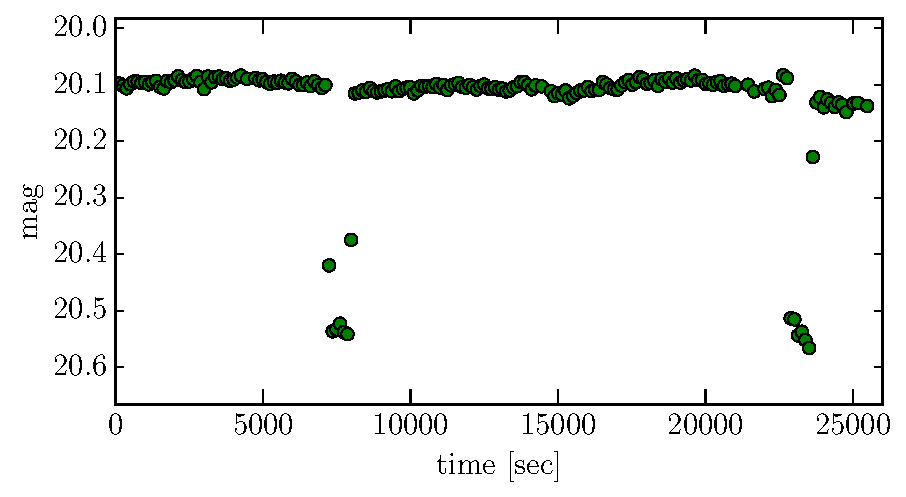
\includegraphics[width=5cm,clip,angle=90]{pic/eclipse/cand_1.pdf}
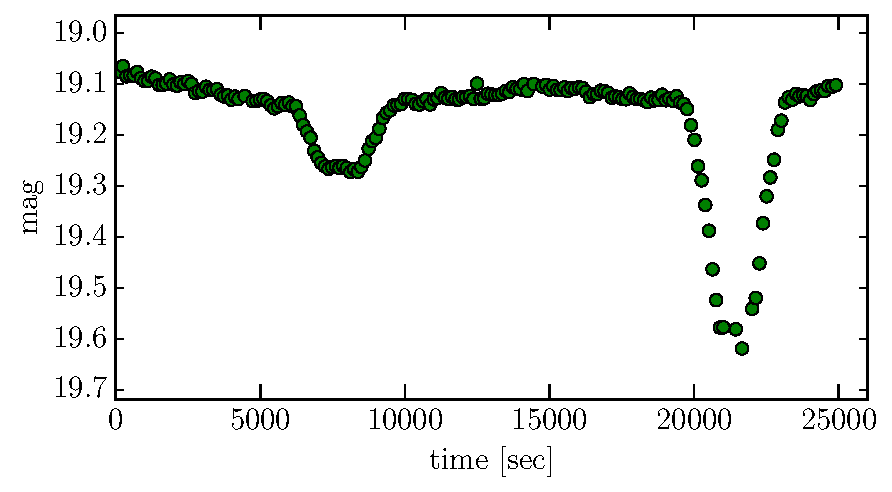
\includegraphics[width=5cm,clip,angle=90]{pic/eclipse/cand_2.pdf}
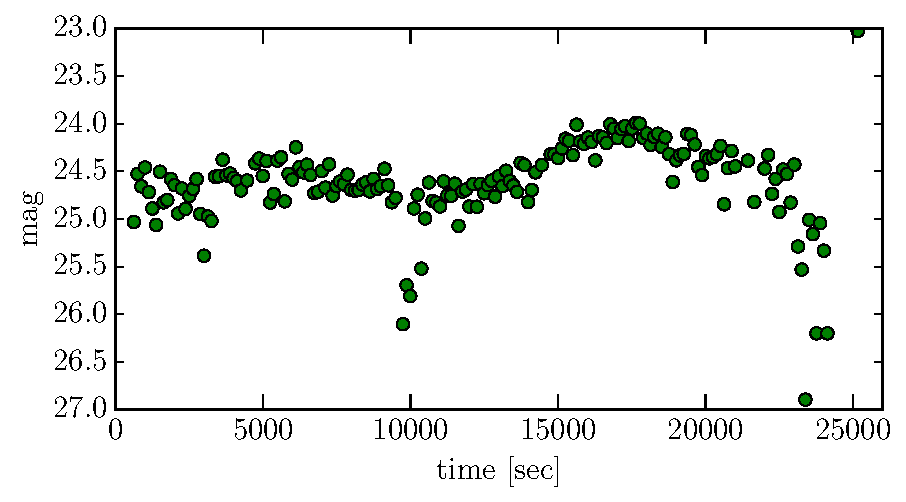
\includegraphics[width=5cm,clip,angle=90]{pic/eclipse/cand_3.pdf}
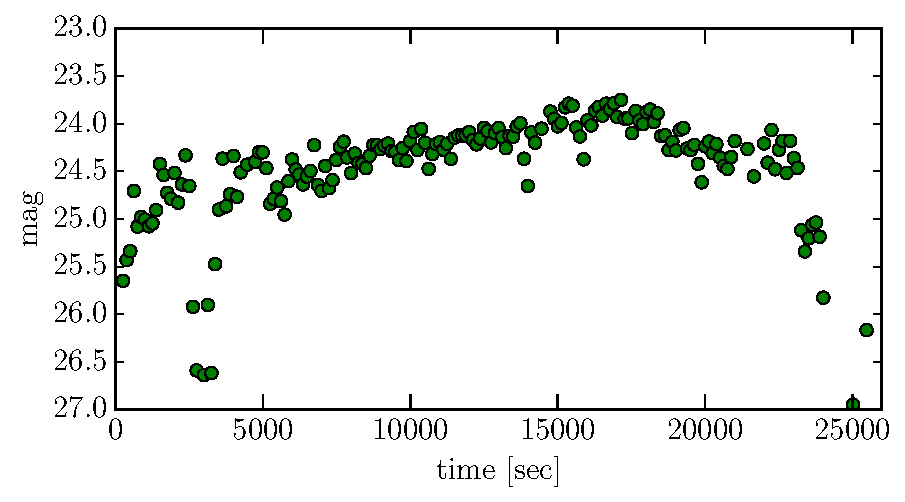
\includegraphics[width=5cm,clip,angle=90]{pic/eclipse/cand_4.pdf}
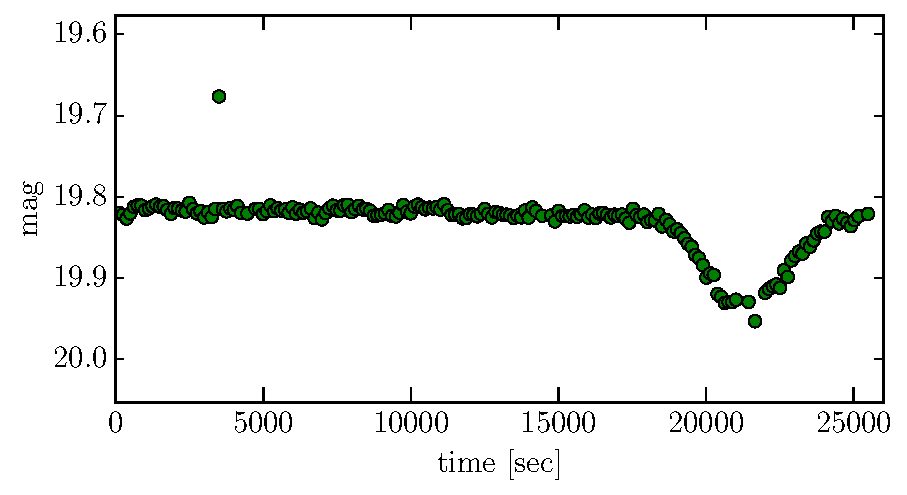
\includegraphics[width=5cm,clip,angle=90]{pic/eclipse/cand_5.pdf}
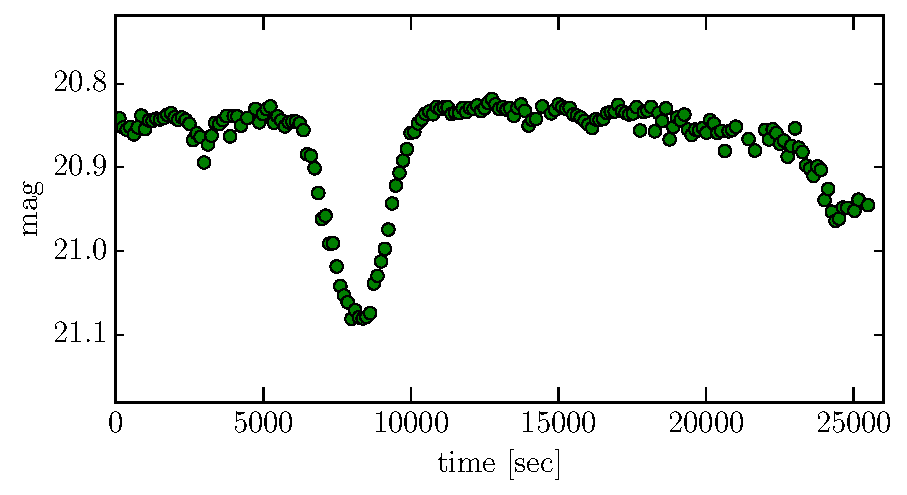
\includegraphics[width=5cm,clip,angle=90]{pic/eclipse/cand_6.pdf}
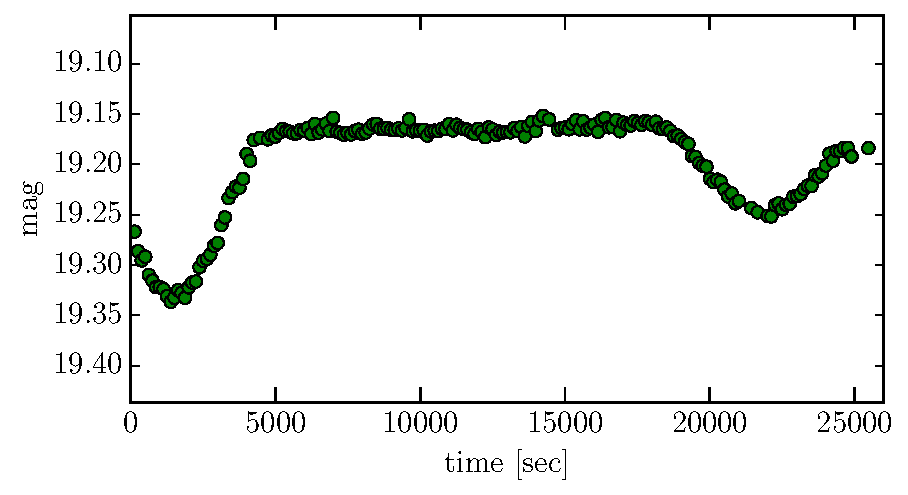
\includegraphics[width=5cm,clip,angle=90]{pic/eclipse/cand_7.pdf}
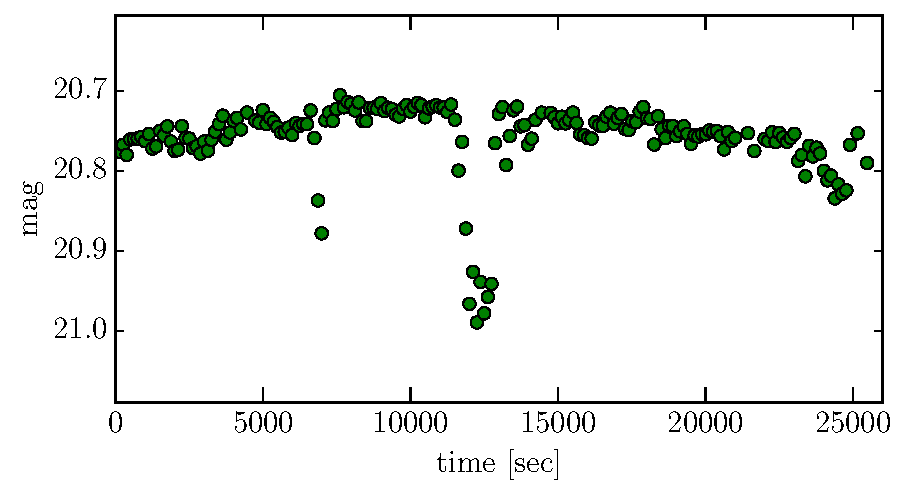
\includegraphics[width=5cm,clip,angle=90]{pic/eclipse/cand_8.pdf}
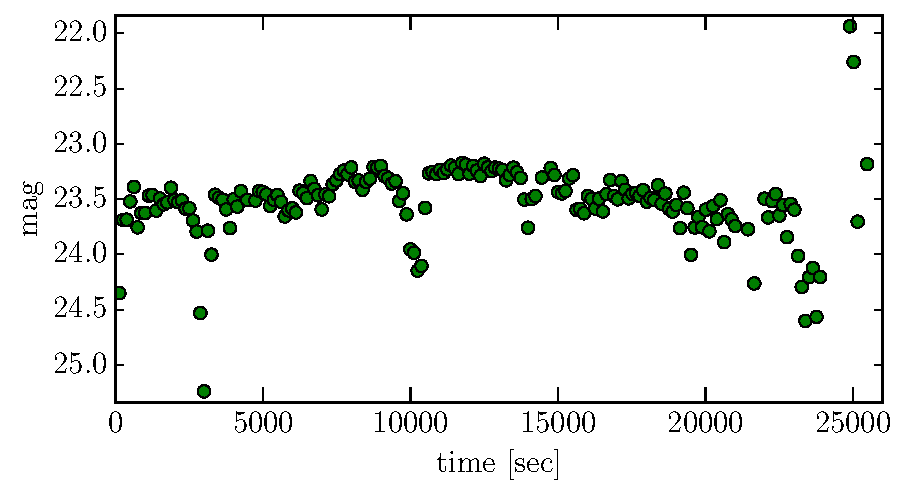
\includegraphics[width=5cm,clip,angle=90]{pic/eclipse/cand_9.pdf}
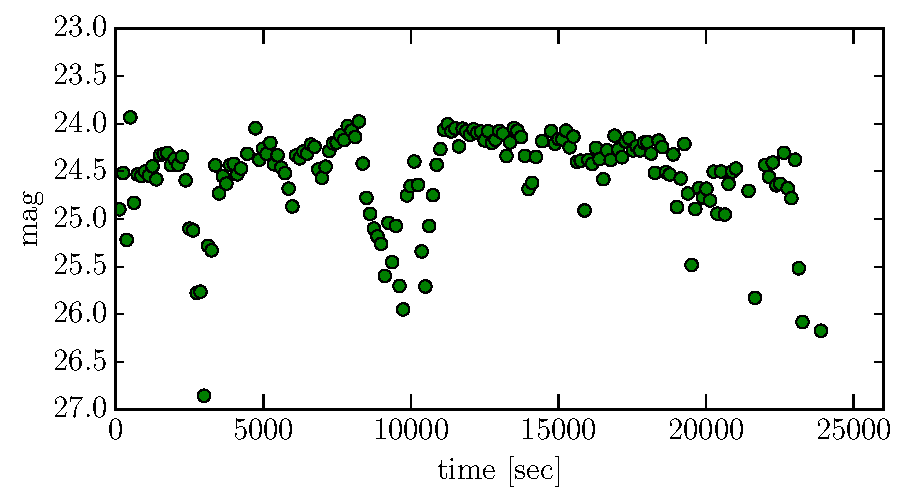
\includegraphics[width=5cm,clip,angle=90]{pic/eclipse/cand_10.pdf}
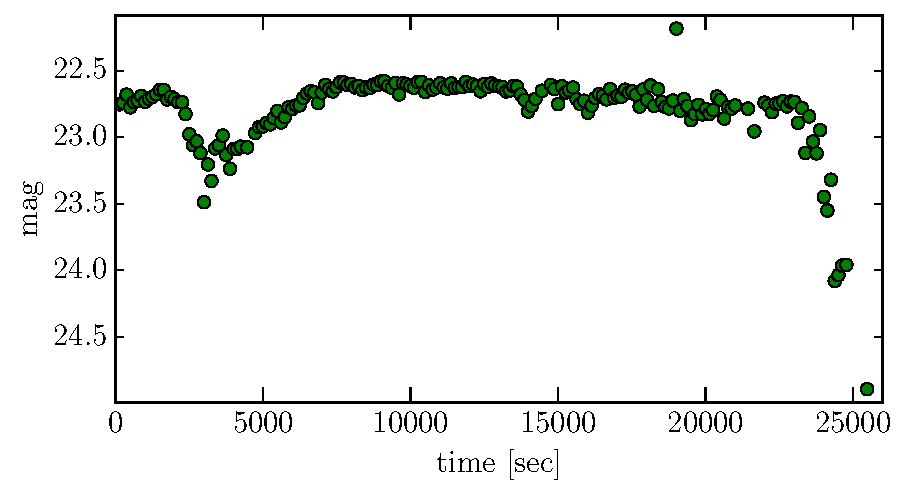
\includegraphics[width=5cm,clip,angle=90]{pic/eclipse/cand_11.pdf}
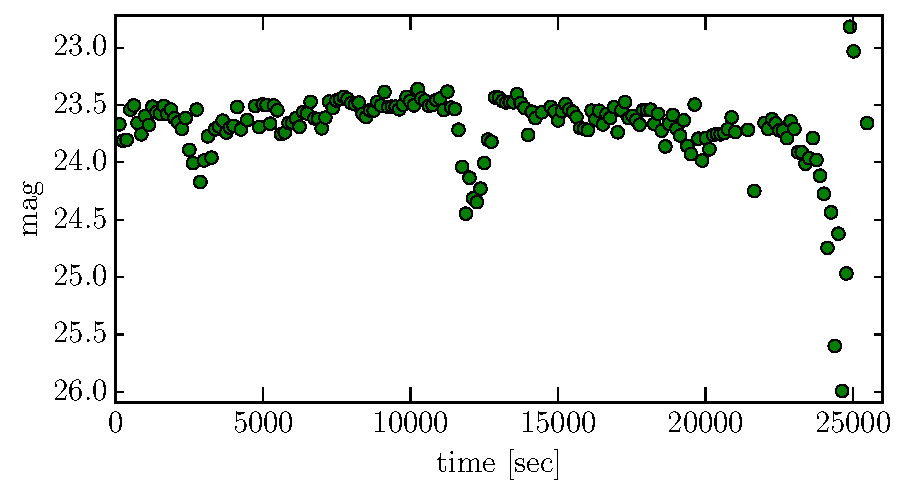
\includegraphics[width=5cm,clip,angle=90]{pic/eclipse/cand_12.pdf}
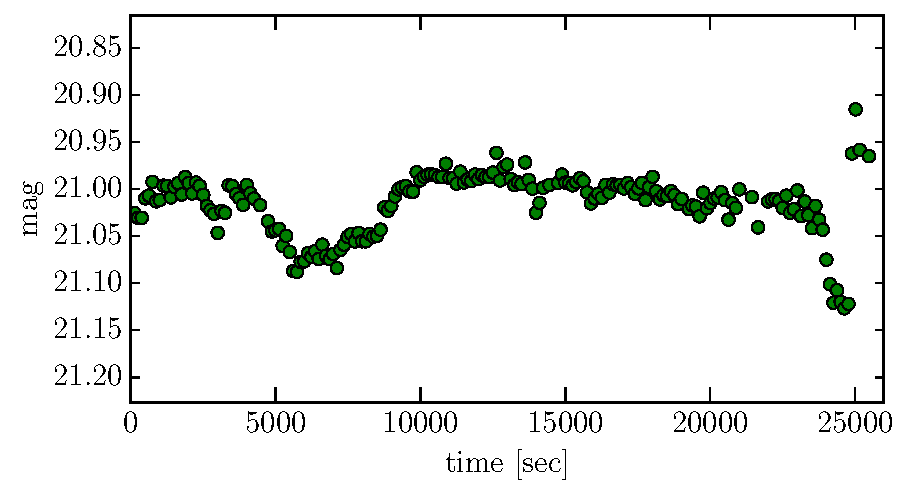
\includegraphics[width=5cm,clip,angle=90]{pic/eclipse/cand_13.pdf}
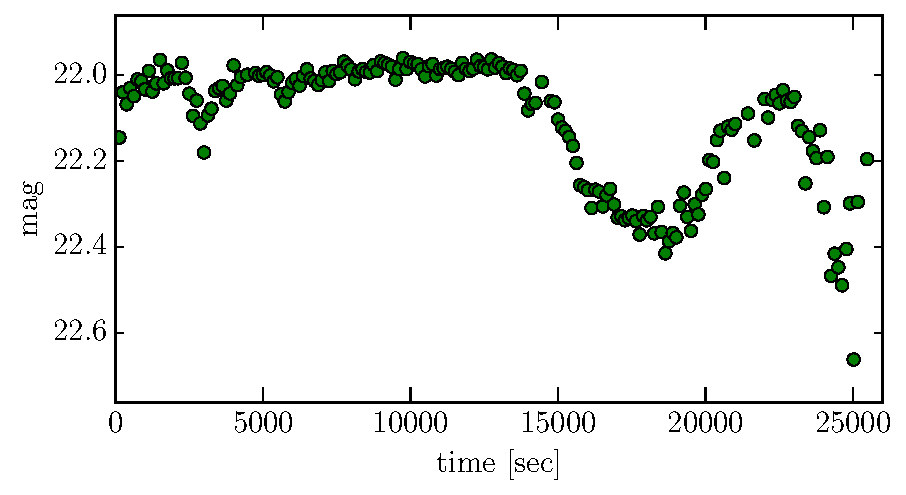
\includegraphics[width=5cm,clip,angle=90]{pic/eclipse/cand_14.pdf}
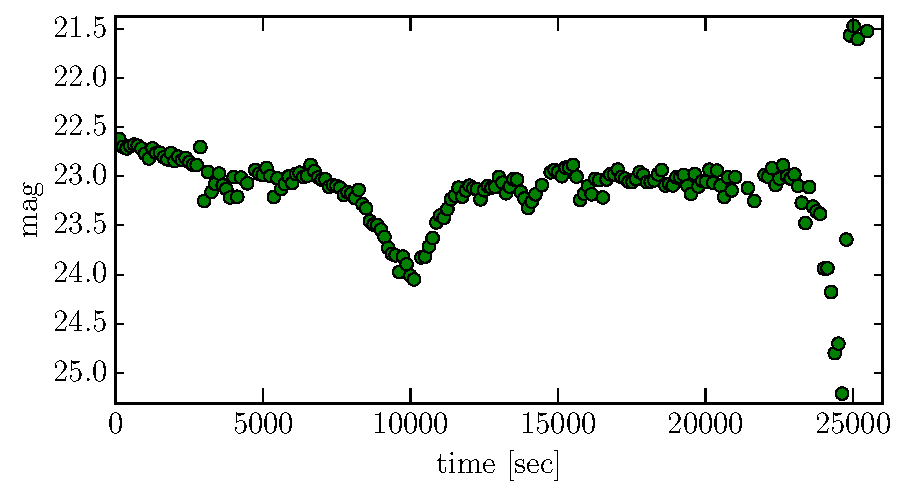
\includegraphics[width=5cm,clip,angle=90]{pic/eclipse/cand_15.pdf}
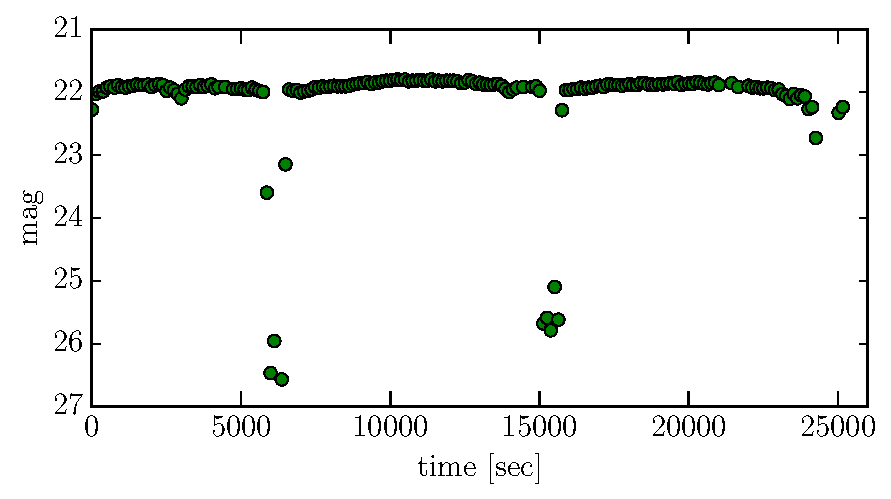
\includegraphics[width=5cm,clip,angle=90]{pic/eclipse/cand_16.pdf}
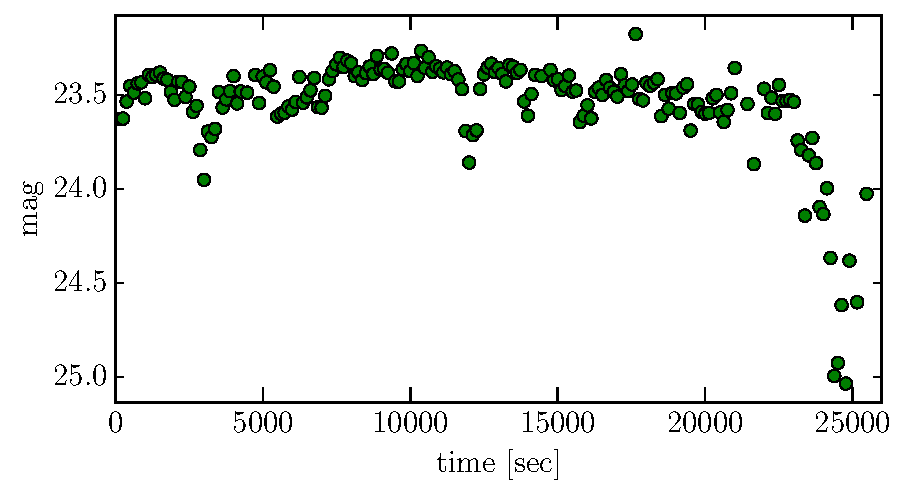
\includegraphics[width=5cm,clip,angle=90]{pic/eclipse/cand_17.pdf}
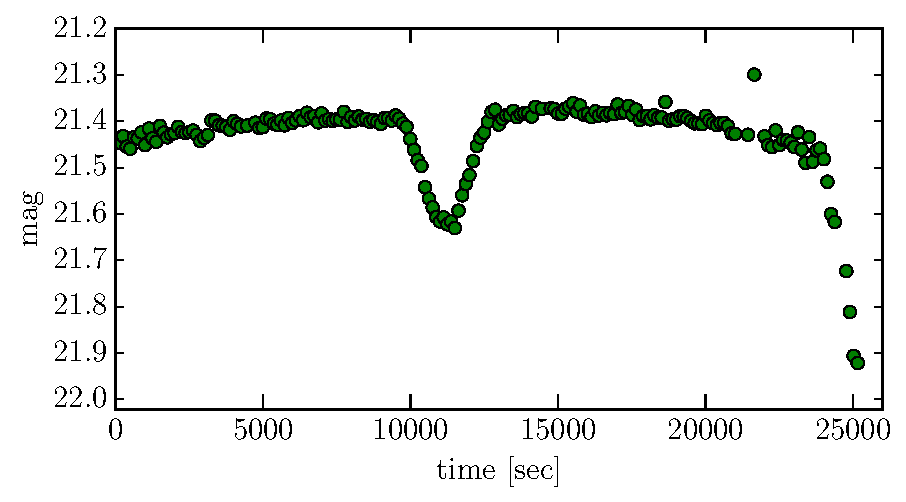
\includegraphics[width=5cm,clip,angle=90]{pic/eclipse/cand_18.pdf}
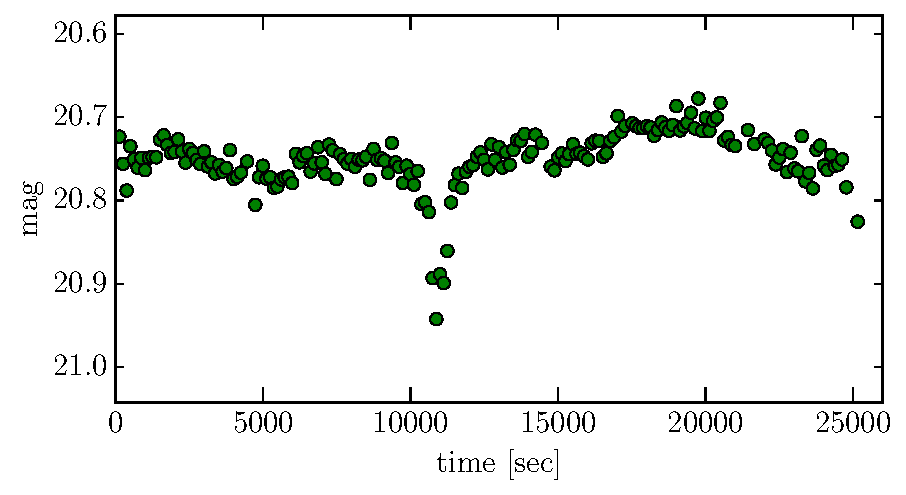
\includegraphics[width=5cm,clip,angle=90]{pic/eclipse/cand_19.pdf}
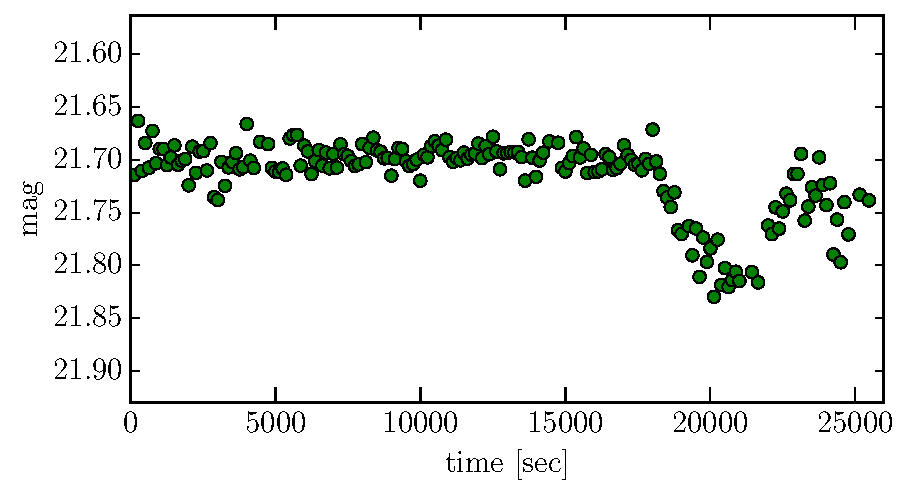
\includegraphics[width=5cm,clip,angle=90]{pic/eclipse/cand_20.pdf}
\includegraphics[width=5cm,clip,angle=90]{pic/eclipse/cand_21.pdf}
\includegraphics[width=5cm,clip,angle=90]{pic/eclipse/cand_22.pdf}
\includegraphics[width=5cm,clip,angle=90]{pic/eclipse/cand_23.pdf}
\includegraphics[width=5cm,clip,angle=90]{pic/eclipse/cand_24.pdf}
\caption{{\small
Light curves of eclipsing binary-star candidates.
}}
\label{fig:candeclipse}
\end{figure}



\clearpage
\section{Binary stars}
\begin{figure}[h]
\centering
%\includegraphics[scale=0.6,clip,angle=0]{pic/candidate_flare.pdf}
%\includegraphics[scale=0.36,clip,angle=0]{pic/candidate_flare2.pdf}
\includegraphics[width=5cm,clip,angle=90]{pic/binary/cand_1.pdf}
\includegraphics[width=5cm,clip,angle=90]{pic/binary/cand_2.pdf}
\includegraphics[width=5cm,clip,angle=90]{pic/binary/cand_3.pdf}
\includegraphics[width=5cm,clip,angle=90]{pic/binary/cand_4.pdf}
\includegraphics[width=5cm,clip,angle=90]{pic/binary/cand_5.pdf}
\includegraphics[width=5cm,clip,angle=90]{pic/binary/cand_6.pdf}
\includegraphics[width=5cm,clip,angle=90]{pic/binary/cand_7.pdf}
\includegraphics[width=5cm,clip,angle=90]{pic/binary/cand_8.pdf}
\includegraphics[width=5cm,clip,angle=90]{pic/binary/cand_9.pdf}
\includegraphics[width=5cm,clip,angle=90]{pic/binary/cand_10.pdf}
\includegraphics[width=5cm,clip,angle=90]{pic/binary/cand_11.pdf}
\includegraphics[width=5cm,clip,angle=90]{pic/binary/cand_12.pdf}
\includegraphics[width=5cm,clip,angle=90]{pic/binary/cand_13.pdf}
\includegraphics[width=5cm,clip,angle=90]{pic/binary/cand_14.pdf}
\includegraphics[width=5cm,clip,angle=90]{pic/binary/cand_15.pdf}
\includegraphics[width=5cm,clip,angle=90]{pic/binary/cand_16.pdf}
\includegraphics[width=5cm,clip,angle=90]{pic/binary/cand_17.pdf}
\includegraphics[width=5cm,clip,angle=90]{pic/binary/cand_18.pdf}
\includegraphics[width=5cm,clip,angle=90]{pic/binary/cand_19.pdf}
\includegraphics[width=5cm,clip,angle=90]{pic/binary/cand_20.pdf}
\includegraphics[width=5cm,clip,angle=90]{pic/binary/cand_21.pdf}
\includegraphics[width=5cm,clip,angle=90]{pic/binary/cand_22.pdf}
\includegraphics[width=5cm,clip,angle=90]{pic/binary/cand_23.pdf}
\includegraphics[width=5cm,clip,angle=90]{pic/binary/cand_24.pdf}
\caption{{\small
Light curves of binary-star candidates.
}}
\label{fig:candbinary}
\end{figure}


\clearpage
\section{Cepheid candidates}
\begin{figure}[h]
\centering
%\includegraphics[scale=0.6,clip,angle=0]{pic/candidate_flare.pdf}
%\includegraphics[scale=0.36,clip,angle=0]{pic/candidate_flare2.pdf}
\includegraphics[width=5cm,clip,angle=90]{pic/cepheid/cand_1.pdf}
\includegraphics[width=5cm,clip,angle=90]{pic/cepheid/cand_2.pdf}
\includegraphics[width=5cm,clip,angle=90]{pic/cepheid/cand_3.pdf}
\includegraphics[width=5cm,clip,angle=90]{pic/cepheid/cand_4.pdf}
\includegraphics[width=5cm,clip,angle=90]{pic/cepheid/cand_5.pdf}
\includegraphics[width=5cm,clip,angle=90]{pic/cepheid/cand_6.pdf}
\includegraphics[width=5cm,clip,angle=90]{pic/cepheid/cand_7.pdf}
\includegraphics[width=5cm,clip,angle=90]{pic/cepheid/cand_8.pdf}
\includegraphics[width=5cm,clip,angle=90]{pic/cepheid/cand_9.pdf}
\includegraphics[width=5cm,clip,angle=90]{pic/cepheid/cand_10.pdf}
\includegraphics[width=5cm,clip,angle=90]{pic/cepheid/cand_11.pdf}
\includegraphics[width=5cm,clip,angle=90]{pic/cepheid/cand_12.pdf}
\includegraphics[width=5cm,clip,angle=90]{pic/cepheid/cand_13.pdf}
\includegraphics[width=5cm,clip,angle=90]{pic/cepheid/cand_14.pdf}
\includegraphics[width=5cm,clip,angle=90]{pic/cepheid/cand_15.pdf}
\includegraphics[width=5cm,clip,angle=90]{pic/cepheid/cand_16.pdf}
\includegraphics[width=5cm,clip,angle=90]{pic/cepheid/cand_17.pdf}
\includegraphics[width=5cm,clip,angle=90]{pic/cepheid/cand_18.pdf}
\includegraphics[width=5cm,clip,angle=90]{pic/cepheid/cand_19.pdf}
\includegraphics[width=5cm,clip,angle=90]{pic/cepheid/cand_20.pdf}
\includegraphics[width=5cm,clip,angle=90]{pic/cepheid/cand_21.pdf}
\includegraphics[width=5cm,clip,angle=90]{pic/cepheid/cand_22.pdf}
\includegraphics[width=5cm,clip,angle=90]{pic/cepheid/cand_23.pdf}
\includegraphics[width=5cm,clip,angle=90]{pic/cepheid/cand_24.pdf}
\caption{{\small
Light curves of cepheid variable-star candidates.
}}
\label{fig:candcepheid}
\end{figure}


\clearpage
\section{Flares}
\begin{figure}[h]
\centering
%\includegraphics[scale=0.6,clip,angle=0]{pic/candidate_flare.pdf}
%\includegraphics[scale=0.36,clip,angle=0]{pic/candidate_flare2.pdf}
\includegraphics[width=5cm,clip,angle=90]{pic/flare/cand_1.pdf}
\includegraphics[width=5cm,clip,angle=90]{pic/flare/cand_2.pdf}
\includegraphics[width=5cm,clip,angle=90]{pic/flare/cand_3.pdf}
\includegraphics[width=5cm,clip,angle=90]{pic/flare/cand_4.pdf}
\includegraphics[width=5cm,clip,angle=90]{pic/flare/cand_5.pdf}
\includegraphics[width=5cm,clip,angle=90]{pic/flare/cand_6.pdf}
\includegraphics[width=5cm,clip,angle=90]{pic/flare/cand_7.pdf}
\includegraphics[width=5cm,clip,angle=90]{pic/flare/cand_8.pdf}
\includegraphics[width=5cm,clip,angle=90]{pic/flare/cand_9.pdf}
\includegraphics[width=5cm,clip,angle=90]{pic/flare/cand_10.pdf}
\includegraphics[width=5cm,clip,angle=90]{pic/flare/cand_11.pdf}
\includegraphics[width=5cm,clip,angle=90]{pic/flare/cand_12.pdf}
\includegraphics[width=5cm,clip,angle=90]{pic/flare/cand_13.pdf}
\includegraphics[width=5cm,clip,angle=90]{pic/flare/cand_14.pdf}
\includegraphics[width=5cm,clip,angle=90]{pic/flare/cand_15.pdf}
\includegraphics[width=5cm,clip,angle=90]{pic/flare/cand_16.pdf}
\includegraphics[width=5cm,clip,angle=90]{pic/flare/cand_17.pdf}
\includegraphics[width=5cm,clip,angle=90]{pic/flare/cand_18.pdf}
\includegraphics[width=5cm,clip,angle=90]{pic/flare/cand_19.pdf}
\includegraphics[width=5cm,clip,angle=90]{pic/flare/cand_20.pdf}
\includegraphics[width=5cm,clip,angle=90]{pic/flare/cand_21.pdf}
\includegraphics[width=5cm,clip,angle=90]{pic/flare/cand_22.pdf}
\includegraphics[width=5cm,clip,angle=90]{pic/flare/cand_23.pdf}
\includegraphics[width=5cm,clip,angle=90]{pic/flare/cand_24.pdf}
\caption{{\small
Light curves of flare-star candidates.
}}
\label{fig:candflare}
\end{figure}


\clearpage
\section{Fake events with common light curves}
\begin{figure}[h]
\centering
%\includegraphics[scale=0.6,clip,angle=0]{pic/candidate_flare.pdf}
%\includegraphics[scale=0.36,clip,angle=0]{pic/candidate_flare2.pdf}
\includegraphics[width=4.9cm,clip,angle=90]{pic/rrlyr/cand_1.pdf}
\includegraphics[width=4.9cm,clip,angle=90]{pic/rrlyr/cand_2.pdf}
\includegraphics[width=4.9cm,clip,angle=90]{pic/rrlyr/cand_3.pdf}
\includegraphics[width=4.9cm,clip,angle=90]{pic/rrlyr/cand_4.pdf}
\includegraphics[width=4.9cm,clip,angle=90]{pic/rrlyr/cand_5.pdf}
\includegraphics[width=4.9cm,clip,angle=90]{pic/rrlyr/cand_6.pdf}
\includegraphics[width=4.9cm,clip,angle=90]{pic/rrlyr/cand_7.pdf}
\includegraphics[width=4.9cm,clip,angle=90]{pic/rrlyr/cand_8.pdf}
\includegraphics[width=4.9cm,clip,angle=90]{pic/rrlyr/cand_9.pdf}
\includegraphics[width=4.9cm,clip,angle=90]{pic/rrlyr/cand_10.pdf}
\includegraphics[width=4.9cm,clip,angle=90]{pic/rrlyr/cand_11.pdf}
\includegraphics[width=4.9cm,clip,angle=90]{pic/rrlyr/cand_12.pdf}
\includegraphics[width=4.9cm,clip,angle=90]{pic/rrlyr/cand_13.pdf}
\includegraphics[width=4.9cm,clip,angle=90]{pic/rrlyr/cand_14.pdf}
\includegraphics[width=4.9cm,clip,angle=90]{pic/rrlyr/cand_15.pdf}
\includegraphics[width=4.9cm,clip,angle=90]{pic/rrlyr/cand_16.pdf}
\includegraphics[width=4.9cm,clip,angle=90]{pic/rrlyr/cand_17.pdf}
\includegraphics[width=4.9cm,clip,angle=90]{pic/rrlyr/cand_18.pdf}
\includegraphics[width=4.9cm,clip,angle=90]{pic/rrlyr/cand_19.pdf}
\includegraphics[width=4.9cm,clip,angle=90]{pic/rrlyr/cand_20.pdf}
\includegraphics[width=4.9cm,clip,angle=90]{pic/rrlyr/cand_21.pdf}
\includegraphics[width=4.9cm,clip,angle=90]{pic/rrlyr/cand_22.pdf}
\includegraphics[width=4.9cm,clip,angle=90]{pic/rrlyr/cand_23.pdf}
\includegraphics[width=4.9cm,clip,angle=90]{pic/rrlyr/cand_24.pdf}
%\includegraphics[width=4.5cm,clip,angle=90]{pic/rrlyr/cand_25.pdf}
\caption{{\small
Light curves of fake candidates which might contain RR-Lyrae variables. 
}}
\label{fig:candrrlyr}
\end{figure}

\end{comment}




\begin{comment}
\section{SUMMARY AND CONCLUSION}
\label{sec:dis2}
In this work we discussed our tests of nature of dark matter on star scales, and 
searched dark matter candidate so-called primordial black hole (PBH). 
We make use of microlensing effect for the search 
which is expected when PBH comes in the line of sight of background stars. 
Microlensing effect is rare event; only one in million stars can happen. 
Thus we used the Hyper Suprime-Cam (HSC) images of Andromeda Galaxy (M31) 
on stars in M31 to gather large number of stars and achieve higher event rate.  
The PBH is one of viable candidates for dark matter, and 
we performed tests to establish a way to constrain 
the abundance of PBHs of mass scales, $10^{-9}$-$10^{-7}M_\odot$, 
with the dense-cadence imaging data from wide-field camera.
One large problem is that 
default analysis mode of HSC-pipe software could not reduce the images with large number of stars; 
which caused troubles as in background subtraction, star catalog construction, 
image difference, and event detection. 
Therefore we managed to establish 
the reduction method as described in \S~\ref{sec:obs2} and \S~\ref{sec:res2}, to extract transient candidates from the images. 

From the reduced images we performed two kinds of analysis: 
transient study and microlensing implication. 
As for transient study we succeeded to extract as much as $\sim11,000$ transient candidates. 
We draw light curves for all the events and classified them 
by peak characteristics, $g$-$r$ color and magnitude. 
These characteristics help us figure out unique candidates  
as well as noise properties. 
The summary of candidate characteristics is provided 
in \S~\ref{sec:res2} and Appendix~\ref{sec:noncelestial} and \ref{sec:unieques}. 
We also started the second analysis; estimating microlensing properties and implication expected from our data.
Currently we could not find any microlensing candidates from the data 
by the fitting of theoretical microlensing light curve. 
Thus we started to estimate the upper limit of mass fraction of PBH to the total dark matter abundance implicated from our data. 
As our data covers large field of view, we need to take into account field-dependent properties 
such as star number counts and extinction. 
Therefore we divided the field of view into $10\times10$ sub-regions.  
In the first step we carefully looked into one single 
patch targeting region (patch=2,6) to reveal the position dependence, 
somehow succeeded to estimate the star number counts in the field.   
Our method constructed for one patch can be basically applied for wider field survey 
simply by considering position dependence and repeating the analysis. 
Also we make sure that our observation achieves 
strongest constraint on the mass fraction by simplified analysis. 

This project is still ongoing, and we might need further investigation of microlensing property. 
Especially disk and bulge region we might need further correction for  
estimating the magnitude or number counts of stars, 
because peak counts might not work for these regions. 
Also for microlensing event from PBHs in M31 halo region, 
we need to estimate the event rate more carefully by taking into account 
so-called finite-source effects or limb-darkening effect, 
which might greatly affect event time-scale estimation \citep[see][for the detail]{Riffeseretal:08}. 


The development achieved in our study can be applied to 
to future new time-space astronomy; aiming at faint, short-timescale events by 
wide-field or short-cadence survey. 
Currently several wide-field deep transient surveys are ongoing or planned not only by HSC, but also by 
the Palomar Transient Factory (PTF)\footnote{http://www.ptf.caltech.edu/iptf} and 
the Large Synoptic Survey Telescope (LSST)\footnote{http://www.lsst.org}. 
As for transient candidates, we can establish clear criteria 
to categorize the events like flares and binary stars including noise characteristics.  
Since our observation presents unique properties of faint, short-timescale variable candidates  
that has never been searched before, 
it would be helpful to characterize the time-dependent behavior of events 
in the future short cadence survey; 
as for microlensing study, event criteria can work as reference to 
remove contamination from microlensing candidates, for example. 
\end{comment}



%%%%%%%%%%%%%%%%%%%%%%%%%%%%%%%%%%%%%%%%%%%%%%%%%%%%%%%%%%%%%%%%%%%%%%%%%%
% ACKNOWLEDGMENTS
%%%%%%%%%%%%%%%%%%%%%%%%%%%%%%%%%%%%%%%%%%%%%%%%%%%%%%%%%%%%%%%%%%%%%%%%%%
\section*{Acknowledgments}

MT was supported by World Premier International Research Center
Initiative (WPI Initiative), MEXT, Japan, by the FIRST program ``Subaru
Measurements of Images and Redshifts (SuMIRe)'', CSTP, Japan. MT was supported 
by Grant-in-Aid for Scientific Research from the JSPS Promotion of Science
(No.~23340061 and 26610058). 

\bibliographystyle{apj}
\bibliography{refs}


\end{document}
